% =====================================================================
%  VoiceGuard — IEEE conference-format paper (DRAFT)
% =====================================================================
%  Compile: this file needs no local LaTeX install.
%  Easiest path: create a new project on https://overleaf.com, choose
%  the "IEEE Conference" template (or any blank project), replace its
%  main.tex with this file's contents, and click Recompile.
%
%  TODO before submission (search for "TODO" below):
%    - author names / affiliations / e-mails
%    - anonymize for double-blind venues (see paper/README.md)
%    - AI-assistance disclosure wording, checked against the target
%      venue's specific policy (see paper/README.md)
%    - expand the reference list for the specific venue's expectations
% =====================================================================
\documentclass[conference]{IEEEtran}
\IEEEoverridecommandlockouts
\usepackage{cite}
\usepackage{amsmath,amssymb,amsfonts}
\usepackage{graphicx}
\usepackage{textcomp}
\usepackage{xcolor}
\usepackage{tikz}
\usetikzlibrary{arrows.meta,positioning,fit,backgrounds}
\usepackage{booktabs}
\usepackage{array}
\usepackage{url}
\usepackage{hyperref}

\def\BibTeX{{\rm B\kern-.05em{\sc i\kern-.025em b}\kern-.08em
    T\kern-.1667em\lower.7ex\hbox{E}\kern-.125emX}}

\begin{document}

\title{VoiceGuard: An Evaluation-Honest, Multi-Signal Decision Layer\\
for Real-Time Voice-Clone Detection in High-Stakes Telephone Calls}

% ---------------------------------------------------------------------
% TODO: replace with the real author list, affiliations and e-mails.
% "Ghanshyam Kumavat" is inferred from the project's git commit
% identity (kumavatghanshyam10@gmail.com) -- confirm the spelling and
% add every teammate before submission.
% ---------------------------------------------------------------------
\author{
\IEEEauthorblockN{Ghanshyam Kumavat\IEEEauthorrefmark{1}, Team Member Two\IEEEauthorrefmark{1}, Team Member Three\IEEEauthorrefmark{1}}
\IEEEauthorblockA{\IEEEauthorrefmark{1}Department of Computer Engineering, \textit{Your Institution Name}, Your City, India\\
Email: \{your.email, teammate2.email, teammate3.email\}@example.edu}
}

\maketitle

\begin{abstract}
Published speech anti-spoofing countermeasures report sub-1\% Equal Error
Rate (EER) on the ASVspoof 2019 benchmark, yet prior work shows this
performance collapses on audio the models were not trained on. We make
three contributions toward closing the gap between benchmark and
deployment for telephone-based voice-clone fraud. First, we identify and
close a silence-duration/loudness shortcut in the standard ASVspoof 2019
LA evaluation pipeline: a classifier trained on unprotected features
scored 13--15\% EER using \emph{only the non-speech regions} of dev
clips (chance is 50\%), meaning part of its apparent accuracy came from
an artifact, not synthesis. We propose a reusable anti-shortcut
front-end and a permanent silence-ablation gate, and re-evaluate a
published countermeasure (AASIST) honestly: its cross-dataset
(In-the-Wild) EER is 35.8\%, far from its  published in-domain figure.
Second, motivated by the finding that no single acoustic detector we
tested generalizes reliably, we design and build VoiceGuard, a
real-time decision layer that fuses acoustic spoof detection with
speaker-consistency (WavLM x-vector), prosodic/behavioral biometrics,
and call-context signals into a policy-driven ALLOW/VERIFY/ESCALATE
decision, with a feature-only, privacy-preserving audit trail. We show
a concrete case where the acoustic signal alone (29/100 risk) would
pass a cloned call, while the fused system escalates it (68/100) because
speaker consistency fails. Third, we report a pilot cross-lingual study
across five Indian languages showing synthetic-speech recall ranging
from 7.5\% (English) to 85\% (Marathi) for the same English-trained
detector -- evidence that multilingual robustness must be measured, not
assumed. We report every result with full provenance and state our
limitations explicitly.
\end{abstract}

\begin{IEEEkeywords}
audio anti-spoofing, voice-clone detection, speaker verification,
sensor fusion, generalization, evaluation methodology, telephony fraud,
multilingual speech, ASVspoof
\end{IEEEkeywords}

% =====================================================================
\section{Introduction}
% =====================================================================

Low-cost, real-time voice cloning has moved from a research curiosity to
a fraud vector. A few seconds of a target's speech, obtained from a
social-media clip or a previous call, is enough for current
text-to-speech (TTS) and voice-conversion (VC) systems to produce
speech that is convincing over a telephone channel. Financial
institutions and call centers that rely on voice as a soft
authentication factor -- for transaction confirmation, beneficiary
changes, or agent verification -- are directly exposed. This is the
problem framing behind Smart India Hackathon problem statement SIH26104,
which asks for a real-time system that detects cloned or synthetic
speech \emph{and} verifies the claimed speaker \emph{and} measures
behavioral anomalies \emph{and} recommends an action, before a
transaction, under a privacy-preserving design.

The academic literature on synthetic-speech detection reports numbers
that suggest the detection half of this problem is close to solved:
countermeasures trained and evaluated on the ASVspoof 2019 Logical
Access (LA) corpus routinely report Equal Error Rates (EER) below 1\%
\cite{aasist}. Independent replications tell a different story. M\"uller
et al.\ show that models trained on ASVspoof-family data lose up to an
order of magnitude in accuracy on found (``In-the-Wild'') audio
\cite{mueller2022generalize}, and a follow-up study attributes most of
this gap to distributional \emph{difference} between generators rather
than to any generator being intrinsically ``harder'' to detect
\cite{mueller2024harder}. Our own experiments, reported in this paper,
reproduce and extend this finding, and additionally show that part of
the historically reported in-domain accuracy on ASVspoof 2019 LA itself
is an artifact of the corpus, not of synthesis.

This paper reports what we built in response to that finding: not a
better single classifier, but (i) an evaluation protocol that removes a
known shortcut and makes every subsequent number trustworthy, and (ii)
a decision system, \emph{VoiceGuard}, that treats acoustic spoof
detection as one of several weak, partly independent signals rather
than as the whole system, fuses them into an auditable, policy-driven
recommendation, and keeps a human in the loop. We view this as the
practically correct response to a field where no detector we evaluated
-- including a second independent, publicly available deepfake-audio
classifier we tested for comparison -- reliably caught a modern
neural-TTS clone in isolation.

\textbf{Contributions.}
\begin{itemize}
\item We identify a silence-duration/loudness shortcut in the ASVspoof
2019 LA evaluation pipeline (Section~\ref{sec:frontend}) and propose an
anti-shortcut front-end plus a permanent silence-ablation gate as a
reusable protocol, stamped with a reproducible fingerprint on every
reported number.
\item We re-evaluate a published countermeasure (AASIST) through this
protocol and report honest in-domain, unseen-attack, per-attack, and
cross-dataset numbers (Section~\ref{sec:results}), including a
silence-only ablation confirming the shortcut is closed.
\item We design and implement VoiceGuard (Section~\ref{sec:system}), a
four-signal fusion architecture (synthetic-voice, speaker consistency,
prosody/behavior, call context) with a scenario-aware policy engine, a
feature-only audit log, and a REST/WebSocket API with an operator
console, and demonstrate a worked case where fusion recovers a miss by
the acoustic signal alone (Section~\ref{sec:worked-example}).
\item We report a pilot multilingual study, IndicCall-Eval, across five
Indian languages, finding an English-trained detector's synthetic-speech
recall varies from 7.5\% to 85\% by target language
(Section~\ref{sec:indic}).
\item We report, as a distinct contribution to reproducibility, the
concrete engineering failures and fixes encountered while building this
system (Section~\ref{sec:lessons}), several of which are not specific
to our codebase.
\end{itemize}

The remainder of this paper is organized as follows.
Section~\ref{sec:related} surveys related work. Section~\ref{sec:problem}
states the threat model and decision problem. Section~\ref{sec:system}
describes the VoiceGuard architecture, including the anti-shortcut
front-end. Section~\ref{sec:setup} describes datasets and metrics.
Section~\ref{sec:results} reports results. Section~\ref{sec:discussion}
discusses findings and limitations. Section~\ref{sec:lessons} reports
lessons learned. Section~\ref{sec:future} outlines future work, and
Section~\ref{sec:conclusion} concludes.

% =====================================================================
\section{Related Work}
\label{sec:related}
% =====================================================================

\subsection{Spoofing Countermeasures and Challenges}
The ASVspoof challenge series established the standard corpora and
protocols for logical-access (TTS/VC), physical-access (replay), and
deepfake countermeasure research. ASVspoof 2019 LA
\cite{asvspoof2019} remains the most widely used training/evaluation
corpus for logical-access countermeasures; ASVspoof 5
\cite{asvspoof5} scales this to crowdsourced data from roughly 2{,}000
speakers and 32 attack algorithms, and adds adversarial attacks. The
Audio Deep synthesis Detection (ADD) challenge series targets
low-quality, partially fake, and adversarially generated audio under
more realistic noise conditions \cite{add2022}. AASIST
\cite{aasist}, the backbone acoustic detector we use, integrates
spectral and temporal graph attention over a raw-waveform front-end and
is, at the time of writing, a standard strong baseline; RawBoost
\cite{rawboost} is a widely adopted raw-waveform augmentation method for
this family of models.

\subsection{Generalization Failures}
A growing body of work shows that in-domain accuracy on ASVspoof-style
benchmarks does not predict real-world performance. M\"uller et al.\
\cite{mueller2022generalize} evaluate countermeasures trained on
ASVspoof 2019 against an independently collected ``In-the-Wild'' set of
celebrity and political speech and report large relative degradations.
A follow-up study decomposes this gap and finds it is driven mainly by
distributional difference between training and test generators, not by
harder acoustics \cite{mueller2024harder}. Pham et al.\ survey the wider
deepfake-speech-detection literature and reach a similar conclusion
about generalization as the field's central open problem
\cite{pham2024survey}. Our work reproduces this generalization gap on a
model we did not train (Section~\ref{sec:results}) and additionally
shows that the in-domain half of the comparison can itself be inflated
by a corpus artifact -- a failure mode that, to our knowledge, is not
addressed by the works above, all of which evaluate on the corpus as
published.

\subsection{Speaker Verification and Voice Biometrics}
Modern speaker verification uses learned embeddings -- x-vectors
\cite{xvectors} and, more recently, embeddings drawn from large
self-supervised speech models such as WavLM \cite{wavlm} -- compared by
cosine similarity against an enrollment utterance. Commercial voice
biometric and telephony-liveness products (e.g., providers offering
real-time voice liveness or voiceprint-blacklist matching for contact
centers) apply this idea operationally, but published, peer-reviewed
detail on their fusion logic and evaluation methodology is limited.
VoiceGuard uses a WavLM x-vector as one input to an explicit,
inspectable fusion and policy layer rather than as a standalone
accept/reject gate.

\subsection{Multilingual and Low-Resource Synthetic Speech}
Nearly all widely used spoofing corpora and countermeasures are
English-centric. IndicSynth \cite{indicsynth} is a large, recent
multilingual synthetic-speech resource spanning 12 low-resource Indian
languages, explicitly motivated by the observation that detectors
trained on one language transfer poorly, and in an uneven, unpredictable
way, to others. Our IndicCall-Eval pilot (Section~\ref{sec:indic}) is
far smaller in scale than IndicSynth but is, to our knowledge, one of
few reported measurements of an English-trained countermeasure's
\emph{synthetic-recall asymmetry} across Indian languages specifically
in a call-center/telephony framing, and we position it as a motivating
pilot for exactly the kind of larger, consented resource IndicSynth
provides.

\subsection{Positioning}
The works above chiefly optimize or evaluate a single detector against
a fixed benchmark. Our contribution is orthogonal: we treat the
benchmark itself as a thing to be audited (Section~\ref{sec:frontend}),
and we treat detection as one signal inside an auditable
security-decision system (Section~\ref{sec:system}) rather than as a
standalone accept/reject classifier. This framing follows from an
empirical premise -- that no single detector we evaluated generalizes
reliably enough to be trusted alone -- rather than from a claim of a
new state-of-the-art detector.

% =====================================================================
\section{Problem Formulation and Threat Model}
\label{sec:problem}
% =====================================================================
We consider a live or recently recorded telephone call in which a
caller requests an action $a$ of consequence -- confirming a payment,
changing a beneficiary, or resetting a credential. The defender
observes an audio stream $x$ from the caller, an enrollment reference
$e$ for the claimed identity (if any), and call metadata $m$ (caller-ID
match, requested amount, channel, prior flags). The attacker's goal is
to have the system accept an instruction while impersonating the
account holder, via a synthetic (TTS/VC) or replayed voice.

We do not assume a single function $f(x)\!\to\!\{\text{real,fake}\}$ can
solve this reliably: Section~\ref{sec:results} shows that even a strong
published detector, evaluated honestly, misses a large fraction of
unseen attacks. We instead pose the problem as a bounded-risk decision:
given signals $S = \{s_{\text{spoof}}, s_{\text{speaker}},
s_{\text{prosody}}, s_{\text{context}}\}$, each in $[0,1]$ with $1$
meaning \emph{more suspicious}, produce an action
$a \in \{\textsc{allow}, \textsc{verify}, \textsc{escalate}\}$ and a
human-readable justification, under scenario-dependent risk tolerance
(Section~\ref{sec:policy}) and a latency budget compatible with a live
call. The design goal is not zero missed detections -- which no
component here achieves -- but a bounded, explainable, auditable
decision that degrades gracefully when any one signal is weak, absent,
or wrong.

% =====================================================================
\section{The VoiceGuard System}
\label{sec:system}
% =====================================================================

\begin{figure*}[t]
\centering
\resizebox{0.96\textwidth}{!}{%
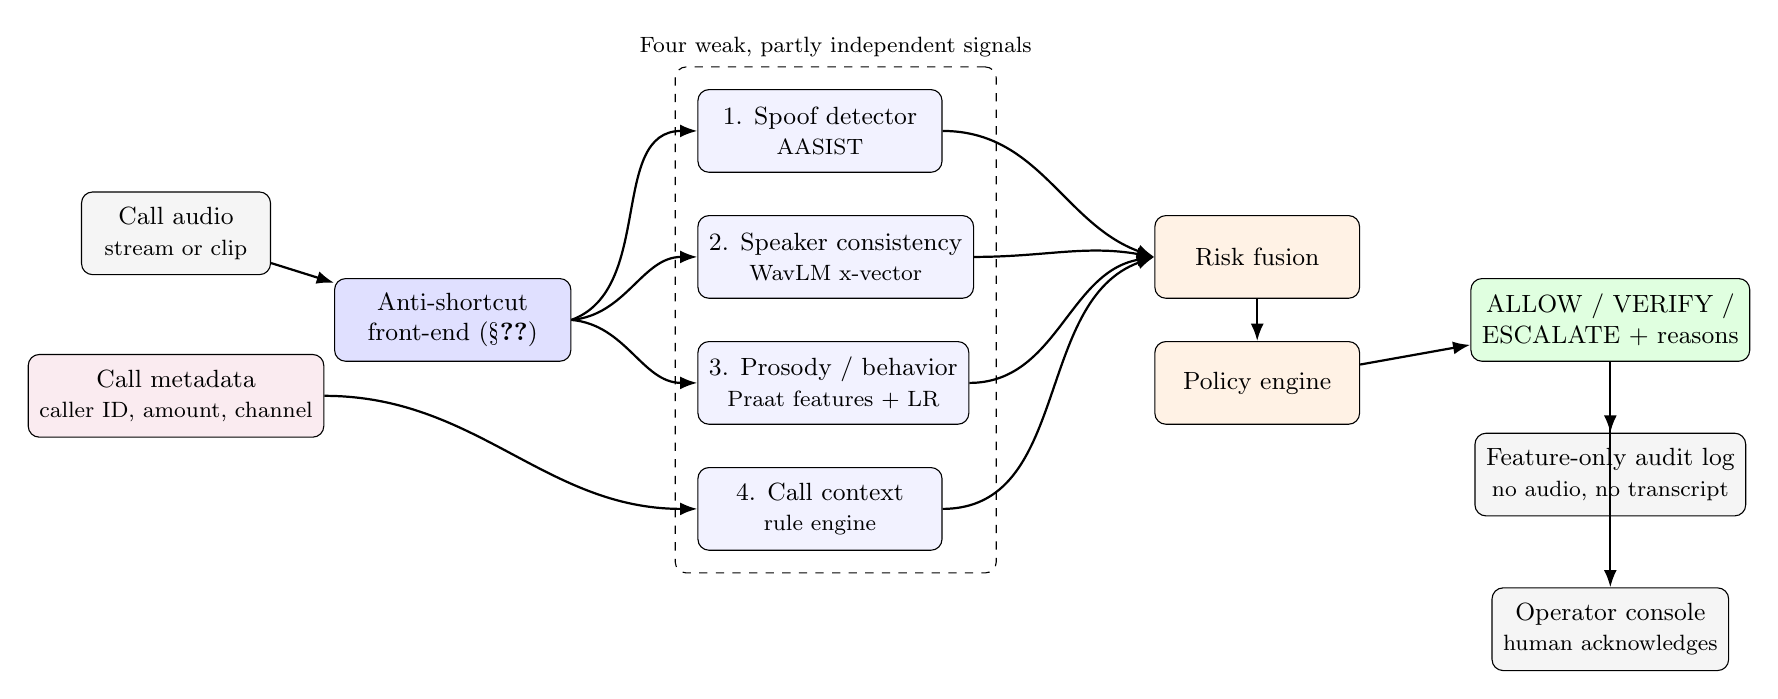
\begin{tikzpicture}[
  node distance=6mm and 8mm,
  box/.style={draw, rounded corners, align=center, minimum height=1.05cm, inner sep=4pt, font=\small},
  sig/.style={box, minimum width=3.1cm, fill=blue!5},
  grp/.style={draw, dashed, rounded corners, inner sep=8pt},
  arr/.style={-{Latex[length=2.2mm]}, thick}
]
  \node[box, minimum width=2.4cm, fill=gray!8] (audio) {Call audio\\\footnotesize stream or clip};
  \node[box, minimum width=2.6cm, fill=purple!8, below=10mm of audio] (meta) {Call metadata\\\footnotesize caller ID, amount, channel};

  \node[box, minimum width=3.0cm, fill=blue!12, right=of audio, yshift=-11mm] (fe) {Anti-shortcut\\front-end (\S\ref{sec:frontend})};

  \node[sig, right=16mm of fe, yshift=24mm] (s1) {1. Spoof detector\\\footnotesize AASIST};
  \node[sig, right=16mm of fe, yshift=8mm]  (s2) {2. Speaker consistency\\\footnotesize WavLM x-vector};
  \node[sig, right=16mm of fe, yshift=-8mm] (s3) {3. Prosody / behavior\\\footnotesize Praat features + LR};
  \node[sig, right=16mm of fe, yshift=-24mm](s4) {4. Call context\\\footnotesize rule engine};

  \node[grp, fit=(s1)(s2)(s3)(s4), label={[font=\footnotesize]above:Four weak, partly independent signals}] (siggrp) {};

  \node[box, minimum width=2.6cm, fill=orange!10, right=20mm of siggrp, yshift=8mm] (fusion) {Risk fusion};
  \node[box, minimum width=2.6cm, fill=orange!10, right=20mm of siggrp, yshift=-8mm] (policy) {Policy engine};

  \node[box, minimum width=2.9cm, fill=green!12, right=14mm of fusion, yshift=-8mm] (decision) {ALLOW / VERIFY /\\ESCALATE + reasons};

  \node[box, minimum width=2.9cm, fill=gray!8, below=9mm of decision] (audit) {Feature-only audit log\\\footnotesize no audio, no transcript};
  \node[box, minimum width=2.9cm, fill=gray!8, below=9mm of audit] (console) {Operator console\\\footnotesize human acknowledges};

  \draw[arr] (audio) -- (fe);
  \draw[arr] (fe.east) to[out=20,in=180]  (s1.west);
  \draw[arr] (fe.east) to[out=5,in=180]   (s2.west);
  \draw[arr] (fe.east) to[out=-5,in=180]  (s3.west);
  \draw[arr] (meta.east) to[out=0,in=180] (s4.west);

  \draw[arr] (s1.east) to[out=0,in=160] (fusion.west);
  \draw[arr] (s2.east) to[out=0,in=170] (fusion.west);
  \draw[arr] (s3.east) to[out=0,in=190] (fusion.west);
  \draw[arr] (s4.east) to[out=0,in=200] (fusion.west);

  \draw[arr] (fusion) -- (policy);
  \draw[arr] (policy) -- (decision);
  \draw[arr] (decision) -- (audit);
  \draw[arr] (decision.south) to[out=-90,in=90] (console.north);
\end{tikzpicture}}
\caption{VoiceGuard architecture. Call audio passes through one
anti-shortcut front-end (Section~\ref{sec:frontend}), shared by every
downstream path. Four signals are computed -- three from audio, one
from call metadata -- and fused with a lone-signal floor
(Section~\ref{sec:fusion}). A scenario-aware policy maps the fused score
to ALLOW/VERIFY/ESCALATE with reason codes, logged to a feature-only
audit trail and surfaced in an operator console.}
\label{fig:architecture}
\end{figure*}

Figure~\ref{fig:architecture} shows the system. We describe each stage
in turn.

\subsection{Anti-Shortcut Evaluation Front-End}
\label{sec:frontend}
Early in this project, a classifier trained on handcrafted acoustic
features and evaluated on the ASVspoof 2019 LA dev split scored an
apparently strong 1.83\% EER. As a sanity check, we re-scored the same
model using \emph{only} the leading and trailing non-speech regions of
each dev clip -- audio that should carry no information about whether
the speaker is genuine or synthetic. The model scored 13--15\% EER on
this silence-only input, far below the 50\% expected of an uninformative
signal. Bona fide and spoof clips in ASVspoof 2019 LA differ
systematically in leading/trailing silence duration and loudness,
almost certainly as a side effect of how the corpus was assembled and
post-processed by different systems; a model can partially solve the
labeling task from this artifact alone, inflating its apparent accuracy
on synthesis detection.

We close this shortcut with a mandatory front-end applied identically
to every clip in every split, for both classes, at feature-extraction,
training, and inference time:
\begin{enumerate}
\item resample to mono, 16\,kHz;
\item trim leading/trailing near-silence and re-pad to a fixed margin,
identically for bona fide and spoof;
\item loudness-normalize to a fixed integrated loudness (EBU R128) and
peak-limit;
\item (optionally) pass through a telephony codec, applied to both
classes when used.
\end{enumerate}
The front-end's configuration is hashed into a short fingerprint
(\texttt{640b0644ae} for every result in this paper) that is stamped on
every reported number; results with different fingerprints are never
compared directly. After every model change, we re-run the silence-only
ablation as a permanent gate: EER on silence-only input must land within
roughly five points of 50\%; below 40\% indicates a reintroduced
shortcut and blocks trusting any other number from that run. We treat
this front-end and gate, not a specific model, as the paper's core
methodological contribution: it is dataset-agnostic and directly reusable by
other ASVspoof 2019 LA work.

\subsection{Signal 1: Synthetic-Voice Detection}
We use AASIST \cite{aasist} with publicly released pretrained weights as
the acoustic spoof-detection signal, run through the front-end above on
a sliding 4.04\,s window with an exponential moving average (EMA) for
the streaming path. We did not train this model ourselves; all numbers
in Section~\ref{sec:results} are for the published checkpoint evaluated
through our protocol. Section~\ref{sec:future} describes our plan to
replace it with a model fine-tuned on modern generators.

\subsection{Signal 2: Speaker Consistency}
A caller enrolls with roughly 6\,s of speech at session start. We embed
both the enrollment audio and each subsequent window with a WavLM
x-vector model (\texttt{wavlm-base-plus-sv} \cite{wavlm}) and compare by
cosine similarity. Similarity is mapped to a risk score by a Platt-scaled
(logistic) calibrator, fit on genuine/impostor trial pairs built from
ASVspoof 2019 LA's real speaker identities and verified, on a
speaker-disjoint held-out split the calibrator never trained on, to
generalize to unseen speakers (Section~\ref{sec:lessons}) -- replacing an
earlier linear interpolation between two hand-picked thresholds, which
remains a fallback when no fitted calibrator is available. Enrollment or
scoring windows shorter than 2.5\,s are rejected as insufficient rather
than scored, because we found that short clips produce spuriously high
similarity regardless of speaker identity (Section~\ref{sec:lessons}).

\subsection{Signal 3: Prosody and Behavioral Biometrics}
We extract 13 prosodic and voice-quality features per window using
Praat/Parselmouth: F0 mean, standard deviation, range and slope; voiced
fraction; jitter (local, RAP); shimmer (local, APQ5); harmonics-to-noise
ratio; intensity variability; pause ratio; and short-term energy flux.
A logistic regression classifier, fit on an ASVspoof 2019 LA training
subset, maps these 13 features to a risk score. This signal is
intentionally weak on its own (Section~\ref{sec:results}); its role is
to contribute evidence that is largely independent of the acoustic
spoof-detection failure modes above.

\subsection{Signal 4: Call Context}
A deterministic rule set scores non-acoustic call metadata: whether the
caller ID matches a known contact, the requested transaction amount
(banded), the channel, and any prior flags on the session. This is the
only signal not derived from audio, and it is the one most directly
under an attacker's non-control -- an attacker with a perfect voice
clone still cannot make an unrecognized number look recognized.

\subsection{Risk Fusion}
\label{sec:fusion}
Let $S \subseteq \{\text{spoof}, \text{speaker}, \text{prosody},
\text{context}\}$ be the signals available for a given window (a signal
is absent before enrollment, or if a scoring window is too short) with
base weights $w_{\text{spoof}}{=}0.45$, $w_{\text{speaker}}{=}0.35$,
$w_{\text{context}}{=}0.20$, $w_{\text{prosody}}{=}0.25$. The fused
score is a weighted mean over present signals with weights renormalized
to sum to one:
\begin{equation}
\text{fused} = \sum_{s \in S} \frac{w_s}{\sum_{s' \in S} w_{s'}}\, \cdot\, \text{score}_s .
\end{equation}
We additionally apply a \emph{lone-signal floor}: if any single present
signal reaches an alarm threshold $\tau_{\text{alarm}}{=}0.80$, the
fused score is floored at $\tau_{\text{floor}}{=}0.68$ regardless of the
weighted mean, so that one strongly suspicious signal cannot be diluted
away by several weakly reassuring ones. Section~\ref{sec:worked-example}
shows this rule firing on real data. On the streaming path, each
signal is additionally smoothed with its own EMA constant, tuned per
signal by observed volatility (Section~\ref{sec:lessons}); the
file-based analysis path used for all results in this paper reports raw,
unsmoothed per-clip scores.

\subsection{Policy Engine}
\label{sec:policy}
A fused score is mapped to an action through a per-scenario threshold
table (Table~\ref{tab:policy}), reflecting that the acceptable
false-escalation rate is not the same for a routine support call as for
a large transfer or a privileged account change. The policy engine also
emits plain-language reason codes built from the individual signals and
context (e.g., ``speaker mismatch: similarity 0.33 vs.\ enrolled voice
(low)'', ``caller number not recognised'', ``large transfer requested
(INR 75{,}000)'') and a recommendation string. Thresholds are documented
operating points, not the output of a calibration procedure
(Section~\ref{sec:discussion}).

\begin{table}[t]
\centering
\caption{Policy thresholds by call scenario (fused score, [0,1])}
\label{tab:policy}
\begin{tabular}{@{}lcc@{}}
\toprule
Scenario & Verify above & Escalate above \\
\midrule
Routine support call    & 0.55 & 0.75 \\
Transaction / transfer  & 0.40 & 0.65 \\
Privileged change       & 0.30 & 0.55 \\
\bottomrule
\end{tabular}
\end{table}

\subsection{Privacy-Preserving Audit Log}
Every action change is written to an append-only JSONL log containing
per-signal scores, the fused score, the action, the reason codes, model
and front-end version, and a git commit hash for provenance. The log
implementation explicitly rejects any write containing an audio,
waveform, transcript, or embedding key, checked recursively, so the
audit trail cannot silently grow to include raw biometric or content
data. This is the system's privacy design, not merely a policy
statement: it is enforced by the logging function's write path.

\subsection{System Interfaces}
A session-oriented REST and WebSocket API exposes session creation,
enrollment, context updates, single-clip analysis, streaming, audit
retrieval, and an acknowledge action for the human operator. A
browser-based operator console renders the decision banner, a fused-risk
timeline, four live signal meters, reason codes, an editable call-context
panel, and the audit trail, so the same decision logic used for the
results in this paper is directly demonstrable end to end. The identical
session API is additionally reachable over gRPC, including a
bidirectional-streaming RPC matching the WebSocket path; both transports
call the same session-management code, and we verify this directly by
asserting that the two transports produce an identical decision and fused
score on the same input clip, rather than only that each responds.

% =====================================================================
\section{Experimental Setup}
\label{sec:setup}
% =====================================================================

\subsection{Datasets and Splits}
We use the official ASVspoof 2019 LA protocol files exclusively: the
training partition for model fitting where applicable, the dev
partition (attacks A01--A06, ``known'') for threshold selection, and the
eval partition (attacks A07--A19, ``unseen'') as an in-domain test. We
additionally use the In-the-Wild corpus \cite{mueller2022generalize} as
a cross-dataset test set that is \emph{never} trained on and never used
to select a threshold. A home-made random split is never used, since it
would leak speakers and attack types across partitions. For the pilot
multilingual study (Section~\ref{sec:indic}), we generate synthetic
attacks in five languages with an open multilingual TTS model
\cite{mms} (Section~\ref{sec:indic}); no bona fide multilingual speech
is included in the numbers reported here (Section~\ref{sec:discussion}).

\subsection{Metrics}
We report Equal Error Rate (EER) as the headline metric, computed at
the standard operating point where false-accept and false-reject rates
are equal, under the convention that higher scores mean more likely
bona fide. We additionally report per-attack EER on the eval partition,
scoring each attack's spoof clips against all bona fide clips
separately, so a single easy attack cannot mask failure on the others,
and min t-DCF (Section~\ref{sec:results}), the ASVspoof challenges' own
deployment-oriented metric, computed with the challenge organizers'
reference implementation against their fixed baseline ASV system so the
number is comparable across papers.
We do not report classification accuracy as a headline number, since
the class prior is roughly 9:1 bona fide:spoof and accuracy is
misleading at that ratio. For the multilingual pilot we report synthetic
recall -- the fraction of generated attacks scored above the system's
synthetic-voice threshold (0.65) -- since no bona fide multilingual set
is yet available to compute a proper EER (Section~\ref{sec:discussion}).

\subsection{Systems Compared}
We compare a Generation-1 baseline (a 61-dimensional handcrafted
acoustic feature set feeding a gradient-boosted-tree ensemble of
XGBoost, LightGBM and CatBoost) against AASIST with published,
pretrained weights, both evaluated through the identical front-end
described in Section~\ref{sec:frontend}. We also implemented, but did
not train to convergence, RawNet2, AASIST-L, and an SSL-AASIST variant
(frozen wav2vec2/XLS-R front-end with a trainable AASIST graph
back-end); a two-epoch sanity run of AASIST on our local GPU (dev EER
34.1\% $\rightarrow$ 26.6\% over two epochs) confirms the training loop
is implemented correctly, but is not a converged model and is not used
for any other result in this paper (Section~\ref{sec:lessons}).

\subsection{Hardware and Reproducibility}
All evaluation was run on a single consumer GPU (6\,GB VRAM). Every
reported row carries a provenance record (train set, test set, model,
seed, front-end fingerprint, score direction, git commit, timestamp),
written automatically by the evaluation harness, so that any number in
this paper can be traced to the exact code and data that produced it.

% =====================================================================
\section{Results}
\label{sec:results}
% =====================================================================

\subsection{Silence-Shortcut Ablation}
Table~\ref{tab:silence} confirms the shortcut identified in
Section~\ref{sec:frontend} is closed after the front-end fix: both the
Generation-1 baseline and AASIST score close to chance (50\%) on
silence-only input, whereas the original, unprotected pipeline scored
13--15\% EER on the same kind of input.

\begin{table}[t]
\centering
\caption{Silence-only ablation after the anti-shortcut fix (chance = 50\%)}
\label{tab:silence}
\begin{tabular}{@{}lc@{}}
\toprule
System & Silence-only EER (\%) \\
\midrule
Handcrafted + GBM ensemble (Gen-1) & 59.0 \\
AASIST (published weights)         & 41.3 \\
\bottomrule
\end{tabular}
\end{table}

\subsection{In-Domain and Cross-Dataset Generalization}
Table~\ref{tab:main} reports our headline result. AASIST, evaluated
honestly through our front-end, scores 9.6\% EER on known attacks and
23.3\% on unseen attacks in-domain -- both markedly higher than the
sub-1\% figures typically reported for this model family, because our
front-end removes the artifact those numbers partly relied on. More
importantly, cross-dataset EER on In-the-Wild is 35.8\%: substantially
worse than in-domain, and far from a deployable figure, though
considerably better than our own Generation-1 baseline's 58.2\% (close
to chance).

\begin{table}[t]
\centering
\caption{Detection performance through the anti-shortcut front-end}
\label{tab:main}
\begin{tabular}{@{}lccc@{}}
\toprule
System & Dev (\%) & Eval (\%) & ITW (\%) \\
 & known & unseen & cross-dataset \\
\midrule
Handcrafted + GBM (Gen-1) & 7.0 & 33.4 & 58.2 \\
AASIST (published weights) & 9.6 & 23.3 & \textbf{35.8} \\
\bottomrule
\end{tabular}
\end{table}

We additionally report min t-DCF (Table~\ref{tab:tdcf}), the ASVspoof
challenges' own deployment-oriented metric: a countermeasure scored in
tandem with a fixed automatic speaker verification (ASV) system under
an explicit cost model, computed with the ASVspoof 2019 organizers'
reference implementation and their baseline ASV system's own scores
(not our speaker-consistency signal) so the number is comparable to
other reported min t-DCF results. It tells the same story as EER,
independently: usable on known attacks (0.288), collapsing on unseen
ones (0.588). We do not compute it against In-the-Wild, which does not
distribute a matching ASV trial list; ASVspoof 2021 DF, a second
held-out cross-dataset test, remains future work
(Section~\ref{sec:future}).

\begin{table}[t]
\centering
\caption{min t-DCF, AASIST through the anti-shortcut front-end}
\label{tab:tdcf}
\begin{tabular}{@{}lcc@{}}
\toprule
System & Dev min-tDCF & Eval min-tDCF \\
 & known & unseen \\
\midrule
AASIST (published weights) & 0.288 & \textbf{0.588} \\
\bottomrule
\end{tabular}
\end{table}

\subsection{Per-Attack Generalization}
Table~\ref{tab:perattack} breaks the unseen-attack (eval) result down
by generator. AASIST is near-perfect on A08/A09 (waveform-concatenation
and neural-vocoder attacks close to its training distribution) but
fails on A10 and A12 (52.1\% and 43.7\% EER respectively) -- unfamiliar
neural TTS/VC systems. This spread, within a single in-domain test
partition, is itself evidence against treating a single aggregate EER
as representative of real-world behavior.

\begin{table}[t]
\centering
\caption{Per-attack EER, eval partition (unseen attacks), AASIST}
\label{tab:perattack}
\begin{tabular}{@{}cccccccc@{}}
\toprule
A07 & A08 & A09 & A10 & A11 & A12 & A13 \\
40.0 & 1.6 & 0.7 & \textbf{52.1} & 17.0 & \textbf{43.7} & 17.7 \\
\midrule
A14 & A15 & A16 & A17 & A18 & A19 & \\
8.0 & 39.0 & 13.7 & 13.7 & 12.4 & 13.4 & \\
\bottomrule
\end{tabular}
\end{table}

\subsection{Prosody Signal, Standalone}
The prosody/behavior logistic-regression classifier
(Section~\ref{sec:system}) scores 26.3\% dev EER on its own -- weak by
design, and weaker than the acoustic signal in isolation. We report it
because its role in this paper is as a contributing, partly independent
fusion input, not as a standalone detector; Section~\ref{sec:worked-example}
shows it contributing correctly (low) on a genuine call.

\subsection{System-Level Worked Example}
\label{sec:worked-example}
Table~\ref{tab:worked} reports a concrete, reproducible case: a session
is enrolled with a genuine speaker, a benign call segment is scored, and
then a call using a different, modern neural-TTS-generated voice is
scored with the call context set to an unrecognized caller and a large
requested transfer (INR 75{,}000). The acoustic spoof signal alone
(29/100) is well below the system's own synthetic-voice threshold
(65/100) -- taken in isolation, the acoustic detector would not flag
this call. The speaker-consistency signal, however, measures a cosine
similarity of 0.33 against the enrolled voice, mapping to a risk of
99/100 and triggering the lone-signal floor
(Section~\ref{sec:fusion}); combined with the context signal, the fused
score reaches 68/100 and the system escalates, with reason codes
including the low speaker-similarity score, the unrecognized caller
number, and the transfer amount. This is, to our knowledge, the clearest
available illustration of the paper's central design argument: a signal
the acoustic detector misses is caught by an orthogonal signal, and the
fusion and floor rules are precisely what make that possible.

\begin{table}[t]
\centering
\caption{Worked example: per-signal risk (0--100) and decision}
\label{tab:worked}
\begin{tabular}{@{}lccccc@{}}
\toprule
Call & Spoof & Spk. & Pros. & Ctx. & Decision (fused) \\
\midrule
Benign & 0 & 44 & 49 & 0 & ALLOW (22) \\
Cloned voice\textsuperscript{a} & 29 & 99 & 20 & 65 & ESCALATE (68) \\
\bottomrule
\end{tabular}
\\[2pt]
\raggedright\footnotesize\textsuperscript{a}Modern neural-TTS clone, unrecognized caller, INR 75{,}000 transfer requested.
\end{table}

The benign call's speaker-consistency reading (44/100) is not zero: two
different recordings of the same person are never a perfect cosine match,
and the calibrated mapping (Section~\ref{sec:system}, Signal 2) reflects
that natural variability rather than collapsing it to zero the way an
uncalibrated threshold would. It stays comfortably inside ALLOW for every
scenario in Table~\ref{tab:policy}.

For comparison, we also tested a second, independently trained,
publicly available deepfake-audio classifier as an alternative acoustic
signal. It performed worse than our front-end-corrected AASIST on both
ASVspoof spoof clips and, notably, missed the modern neural-TTS clone in
Table~\ref{tab:worked} entirely -- reinforcing that the gap is not
specific to AASIST, and that model-shopping for a single better acoustic
detector is not, on present evidence, a substitute for fusion.

\subsection{IndicCall-Eval: A Multilingual Pilot}
\label{sec:indic}
SIH26104 explicitly asks for Indian-language support. Rather than assume
transfer from an English-trained detector, we measured it. We generated
short bank-call-style synthetic-speech attacks with an open multilingual
TTS model \cite{mms} in English, Hindi, Tamil, Bengali, and Marathi (40
clips per language, native script, half passed through a randomly
chosen telephony codec), and scored every clip with the same
AASIST-based detector and threshold used throughout this paper.
Table~\ref{tab:indic} reports synthetic recall -- the fraction of
generated attacks flagged -- per language.

\begin{table}[t]
\centering
\caption{IndicCall-Eval pilot: synthetic-speech recall by language (n=40/language, threshold 0.65)}
\label{tab:indic}
\begin{tabular}{@{}lc@{}}
\toprule
Language & Synthetic recall (\%) \\
\midrule
Marathi  & \textbf{85.0} \\
Hindi    & 57.5 \\
Tamil    & 55.0 \\
Bengali  & 37.5 \\
English  & \textbf{7.5} \\
\bottomrule
\end{tabular}
\end{table}

The result is counter-intuitive and, we believe, informative: the
detector, trained only on English ASVspoof 2019 data, flags
Indian-language synthetic speech \emph{more} often than English
synthetic speech from the same TTS system. We interpret this as evidence
that non-English synthesis sits further, in acoustic-feature space, from
the ``natural English speech'' distribution the model implicitly
learned as its bona fide class, so its artifacts are more likely to trip
a detector tuned on that distribution -- not as evidence of genuine
multilingual robustness. Section~\ref{sec:discussion} discusses why this
is a recall measurement, not an EER, and what would be needed to turn it
into one.

% =====================================================================
\section{Discussion}
\label{sec:discussion}
% =====================================================================

\textbf{The silence-shortcut finding generalizes beyond this project.}
Any evaluation on ASVspoof 2019 LA that does not equalize
leading/trailing silence and loudness across classes is at risk of the
same inflation we measured (13--15\% EER from silence alone). Because
this is a property of a widely used public corpus rather than of our
code, we believe the anti-shortcut front-end and the permanent
silence-ablation gate (Section~\ref{sec:frontend}) are directly useful
to other work using this corpus, independent of our system.

\textbf{Fusion compensates for, but does not fix, a weak acoustic
signal.} The worked example in Section~\ref{sec:worked-example} shows
fusion recovering a miss, but this depended on the speaker-consistency
signal being strong evidence in that specific case (a low-similarity
voice clone). An attacker who additionally spoofed or evaded the
caller-ID check and used a clone similar enough to pass speaker
verification would not be caught by this example's mechanism; we do not
claim the current signal set is sufficient against an adaptive attacker,
only that it catches more than any one signal alone on the cases we
measured.

\textbf{The IndicCall-Eval asymmetry is a recall number, not an EER,
and should not be over-read.} Because we do not yet have a consented
bona fide multilingual speech set, Table~\ref{tab:indic} cannot be
converted into a proper per-language EER, and a high recall number
under a single fixed threshold says nothing about the corresponding
false-accept rate on genuine non-English speech. The pilot's value is
narrower and more honest: it demonstrates that multilingual transfer is
uneven and must be measured per language, and it motivates exactly the
larger, consented resource that concurrent work such as IndicSynth
\cite{indicsynth} provides at a scale far beyond our pilot.

\subsection{Limitations}
We state these explicitly. (1) All detection numbers use a published,
not self-trained, acoustic model; 35.8\% cross-dataset EER is not a
deployable figure. (2) Fusion weights and policy thresholds remain
documented operating points, tuned by inspection. Of the three learned
signals, only speaker consistency is now calibrated on held-out data
(Section~\ref{sec:lessons}); spoof and prosody calibration were measured,
not assumed, and found not to generalize past the data they were fit on,
so both remain uncalibrated by deliberate choice rather than by omission.
(3) The acoustic
model still needs its full 4.04\,s window for a confirmed read, slower
than a sub-2\,s first-read target for a live call; a lightweight
first-pass model for a genuinely shorter confirmed read is not
implemented. We do report latency from speech onset rather than call
connect, and a provisional-read path with a hard safety cap (any read
built from a short or tiled window is capped at a VERIFY action, never
allowed to silently reach the top ESCALATE action, until a full window
confirms it), which closes the honesty gap but not the latency gap
itself. (4) Alerts in the operator console
are simulated; no production SMS/email/webhook sink is wired. (5) The
IndicCall-Eval pilot uses only synthetic attacks from one open TTS
family, at $n{=}40$ per language, and lacks a bona fide multilingual
slice (Section~\ref{sec:indic}). (6) We have not measured performance
under an adaptive attacker aware of the fusion logic. (7) We report
min t-DCF alongside EER, using the
ASVspoof 2019 organizers' own reference implementation and baseline ASV
system so the number is comparable across papers; ASVspoof 2021 DF as a
second, held-out cross-dataset test remains future work
(Section~\ref{sec:future}) -- the corpus requires a registration step
with the organizers we have not completed.

% =====================================================================
\section{Practical Challenges and Lessons Learned}
\label{sec:lessons}
% =====================================================================
We report the following as reproducibility-relevant findings in their
own right, several of which are not specific to our codebase.

\textbf{A corpus can leak the label through non-speech audio.} Already
discussed in Section~\ref{sec:frontend}; this was the single most
consequential finding of the project and the reason every other result
in this paper carries a front-end fingerprint and a permanent ablation
gate.

\textbf{Self-supervised checkpoints can silently fail to load across
library versions.} We found that a WavLM speaker-verification checkpoint's
positional-convolution layer, stored in the older \texttt{weight\_g}/
\texttt{weight\_v} weight-normalization format, loaded without error but
with randomly initialized weights under a newer version of the
\texttt{transformers} library that switched to a \texttt{parametrizations}-based
API -- silently degrading same-speaker cosine similarity, with no
exception raised. The fix was to copy the raw weights from the
checkpoint file into the new parametrization API explicitly at load
time. We flag this because a silent numerical degradation of this kind
is easy to miss without a same-speaker/different-speaker sanity check.

\textbf{Short enrollment or scoring clips produce spuriously confident
speaker matches.} Below roughly 2.5\,s, cosine similarity from the
x-vector embedding became an unreliable indicator of speaker identity;
we added an explicit minimum-duration gate rather than trusting the
similarity score at any duration.

\textbf{A single global smoothing constant destabilizes a fused,
streaming decision.} An early version applied one exponential-smoothing
constant to every signal on the live streaming path; the prosody
signal's higher natural volatility caused the fused decision to
oscillate between ALLOW and VERIFY on stable audio. Per-signal EMA
constants, chosen by each signal's observed volatility, resolved this;
we note it as a general caution for any system fusing signals of
different natural time-scales.

\textbf{Model-shopping is not a substitute for fusion.} We evaluated a
second, independently published deepfake-audio detector as a candidate
replacement acoustic signal. It underperformed our front-end-corrected
AASIST on ASVspoof spoof clips and missed the modern-TTS clone used in
Section~\ref{sec:worked-example} entirely. We take this as evidence
against the strategy of searching for a single better off-the-shelf
detector in place of building a system that does not depend on any one
detector being sufficient.

\textbf{Calibration inherits detection's generalization problem.} We fit
Platt and isotonic calibrators for all three learned signals (spoof,
prosody, speaker) on held-out data and measured Expected Calibration
Error (ECE) and Brier score before and after, rather than assuming a fit
that looks good on its own fitting split is trustworthy. For spoof and
prosody, both methods roughly halved ECE on the split they were fit on
(ASVspoof dev) and made it \emph{worse} on eval (unseen attacks) and,
for spoof, worse again on In-the-Wild (cross-dataset) -- isotonic's dev
ECE collapsed to within $10^{-6}$ of zero while its eval/cross-dataset
ECE rose, a textbook overfitting signature repeated independently in two
signals. We ship neither. The speaker-consistency signal is the
exception: because same/different-speaker cosine-similarity geometry is
comparatively stable (a standard speaker-verification calibration
problem) rather than shifting with an adversarial generator distribution,
a Platt fit on ASVspoof's real speaker identities cut held-out (unseen
speaker) ECE from 0.39 to 0.18 -- ship it, and Section~\ref{sec:system}
(Signal 2) reflects it. We read the contrast itself as evidence for this
paper's thesis: the failure mode here is specifically about generalizing
to \emph{unseen generators}, not a generic "these scores are just
uncalibrated" story that a fit would fix everywhere.

\textbf{Full training does not fit commodity hardware at this corpus's
scale.} A single training epoch over ASVspoof 2019 LA took 50--57
minutes on our 6\,GB laptop GPU; a real run (30--40 epochs) is several
days, and our development machine could run only one such job at a
time. A two-epoch run (Section~\ref{sec:setup}) confirmed the training
code is correct but is not a substitute for a full run; we moved
full training to free cloud GPU compute (Section~\ref{sec:future})
rather than report an under-trained model as a result.

\textbf{Dataset-library churn broke a planned data-collection path
mid-project.} A major version of the \texttt{datasets} library dropped
support for script-based dataset loaders, breaking our planned use of
two public speaker-embedding/multilingual-speech resources. We adapted
by generating speaker-conditioning vectors synthetically for one TTS
path and deferring a real bona fide multilingual set to a smaller,
directly consented team recording effort (Section~\ref{sec:future})
rather than depending on an external pipeline that had just changed
under us.

% =====================================================================
\section{Future Work}
\label{sec:future}
% =====================================================================
\textbf{Trained acoustic model.} Replace the published AASIST weights
with a version fine-tuned on modern neural-TTS output (including
generators not present in ASVspoof 2019), using free cloud GPU compute;
target under 15\% cross-dataset EER, adopted only if it beats the
current published-weights baseline under the identical evaluation
protocol of Section~\ref{sec:frontend}.
\textbf{Calibration.} Speaker consistency is now calibrated
(Section~\ref{sec:lessons}); spoof and prosody were measured and found
not to generalize with a naive dev-set fit -- worth another pass with a
fitting set that spans both known and unseen attacks, or a
domain-conditional calibrator, neither attempted here. The policy
thresholds of Table~\ref{tab:policy} and the context signal remain
uncalibrated operating points.
\textbf{Latency.} A speech-onset voice-activity-detection gate and a
safety-capped provisional-read path now ship (Section~\ref{sec:discussion}),
closing the honesty gap between what the console shows and how
confirmed a read is; a genuinely sub-2\,s \emph{confirmed} read still
needs a second, short-window model to replace or supplement the
current 4.04\,s-window AASIST, not attempted here.
\textbf{Consented multilingual bona fide data.} Extend IndicCall-Eval
with a small, consented, recorded bona fide slice per language so that
Table~\ref{tab:indic}'s recall numbers become proper per-language EERs;
scale toward resources such as IndicSynth \cite{indicsynth}.
\textbf{ASVspoof 2021 DF.} min t-DCF alongside EER now ships
(Section~\ref{sec:discussion}); ASVspoof 2021 DF as a second, held-out
cross-dataset test remains future work, blocked on a registration step
with the corpus organizers.
\textbf{Adaptive-attacker evaluation.} Measure system behavior when an
attacker has knowledge of the fusion logic and specifically targets the
weakest present signal.
\textbf{Production hardening.} A gRPC streaming interface and a model card
now ship (Section~\ref{sec:system}, Section~\ref{sec:discussion});
remaining: real alert delivery (SMS/email/webhook, currently simulated in
the operator console), edge/on-device inference, and authentication/TLS
for both the REST and gRPC servers, which today bind to localhost only by
design, not yet as a closed gap.

% =====================================================================
\section{Conclusion}
\label{sec:conclusion}
% =====================================================================
We set out to build a voice-clone detector and found, first, that a
widely used benchmark for this task can be partially solved by an
artifact unrelated to synthesis, and second, that even after removing
that artifact, a strong published detector generalizes poorly enough
(35.8\% cross-dataset EER) that it should not be deployed alone. Rather
than continue searching for a single better classifier, we built
VoiceGuard around the opposite premise: fuse several weak, partly
independent signals -- acoustic, speaker-consistency, prosodic, and
contextual -- into a policy-driven, auditable decision, and keep a human
in the loop. We showed this design concretely recovering a case the
acoustic signal alone would have missed, and we reported, alongside our
results, the specific engineering failures encountered building the
system, in the belief that an honest account of what did not work the
first time is as reusable to the field as the numbers that did.

% =====================================================================
\section*{Acknowledgment}
% =====================================================================
% TODO: adjust wording to match the target venue's specific
% generative-AI disclosure policy; see paper/README.md.
Portions of this manuscript's drafting, literature search, and LaTeX
formatting were assisted by an AI writing assistant (Claude, Anthropic).
All experiments, measurements, system design, and conclusions are the
authors' own work, verified against the project's source code and
logged results. We thank the Smart India Hackathon SIH26104 problem
statement setters for the problem framing that motivated this work.

% =====================================================================
\begin{thebibliography}{13}

\bibitem{mueller2022generalize}
N.~M. M\"uller, P.~Czempin, F.~Dieckmann, A.~Froghyar, and K.~B\"ottinger,
  ``Does audio deepfake detection generalize?,'' in \emph{Proc.
  Interspeech}, 2022. [Online]. Available: arXiv:2203.16263.

\bibitem{aasist}
J.~Jung, H.-S. Heo, H.~Tak, H.~Shim, J.~S. Chung, B.-J. Lee, H.-J. Yu,
  and N.~Evans, ``AASIST: Audio anti-spoofing using integrated
  spectro-temporal graph attention networks,'' in \emph{Proc. IEEE
  ICASSP}, 2022. [Online]. Available: arXiv:2110.01200.

\bibitem{asvspoof2019}
X.~Wang \emph{et al.}, ``ASVspoof 2019: A large-scale public database of
  synthesized, converted and replayed speech,'' \emph{Computer Speech \&
  Language}, vol.~64, 2020. [Online]. Available: arXiv:1911.01601.

\bibitem{asvspoof5}
X.~Wang, H.~Delgado, H.~Tak, J.~Jung, H.~Shim, M.~Todisco, I.~Kukanov,
  X.~Liu, M.~Sahidullah, T.~Kinnunen, N.~Evans, K.~A. Lee, and
  J.~Yamagishi, ``ASVspoof 5: Crowdsourced speech data, deepfakes, and
  adversarial attacks at scale,'' in \emph{Proc. ASVspoof 5 Workshop
  (Interspeech Satellite)}, 2024. [Online]. Available: arXiv:2408.08739.

\bibitem{mueller2024harder}
N.~M. M\"uller, N.~Evans, H.~Tak, P.~Sperl, and K.~B\"ottinger, ``Harder
  or different? Understanding generalization of audio deepfake
  detection,'' in \emph{Proc. Interspeech}, 2024. [Online]. Available:
  arXiv:2406.03512.

\bibitem{rawboost}
H.~Tak, M.~Kamble, J.~Patino, M.~Todisco, and N.~Evans, ``RawBoost: A
  raw data boosting and augmentation method for speech anti-spoofing,''
  in \emph{Proc. IEEE ICASSP}, 2022. [Online]. Available:
  arXiv:2111.04433.

\bibitem{wavlm}
S.~Chen \emph{et al.}, ``WavLM: Large-scale self-supervised pre-training
  for full stack speech processing,'' \emph{IEEE J. Sel. Topics Signal
  Process.}, vol.~16, no.~6, 2022. [Online]. Available: arXiv:2110.13900.

\bibitem{xvectors}
D.~Snyder, D.~Garcia-Romero, G.~Sell, D.~Povey, and S.~Khudanpur,
  ``X-vectors: Robust DNN embeddings for speaker recognition,'' in
  \emph{Proc. IEEE ICASSP}, 2018.

\bibitem{mms}
V.~Pratap \emph{et al.}, ``Scaling speech technology to 1,000+
  languages,'' 2023. [Online]. Available: arXiv:2305.13516.

\bibitem{indicsynth}
D.~V. Sharma, V.~Ekbote, and A.~Gupta, ``IndicSynth: A large-scale
  multilingual synthetic speech dataset for low-resource Indian
  languages,'' in \emph{Proc. ACL}, 2025.

\bibitem{pham2024survey}
L.~Pham, P.~Lam, D.~Tran, H.~Tang, T.~Nguyen, A.~Schindler, F.~Skopik,
  A.~Polonsky, and C.~Vu, ``A comprehensive survey with critical
  analysis for deepfake speech detection,'' 2024. [Online]. Available:
  arXiv:2409.15180.

\bibitem{add2022}
J.~Yi, R.~Fu, J.~Tao, S.~Nie \emph{et al.}, ``ADD 2022: The first audio
  deep synthesis detection challenge,'' in \emph{Proc. IEEE ICASSP},
  2022. [Online]. Available: arXiv:2202.08433.

\bibitem{sun2023vocoder}
C.~Sun, S.~Jia, S.~Hou, and S.~Lyu, ``AI-synthesized voice detection
  using neural vocoder artifacts,'' in \emph{Proc. IEEE/CVF CVPR
  Workshops}, 2023. [Online]. Available: arXiv:2304.13085.

\end{thebibliography}

\end{document}
